\documentclass[11pt,a4paper]{article}
\usepackage[T1]{fontenc}
\usepackage{lmodern}
\usepackage[margin=2.2cm]{geometry}
\usepackage{amsmath,amssymb}
\usepackage{booktabs,tabularx,array}
\usepackage{graphicx}
\usepackage{float}
\usepackage{longtable}
\usepackage{xcolor}
\usepackage{tikz}
\usetikzlibrary{arrows.meta,positioning}
\usepackage[hidelinks]{hyperref}
\def\sectionautorefname{Section}\def\subsectionautorefname{Section}

\definecolor{navy}{HTML}{1F3A5F}
\definecolor{soft}{HTML}{EEF3FA}
\definecolor{todo}{HTML}{FDF1E9}
\definecolor{todoline}{HTML}{EB6834}
\newcommand{\code}[1]{\texttt{\small #1}}
% A box the author fills in: the course does not allow LLM-written analysis or conclusions.
\newcommand{\authorbox}[2]{\par\smallskip\noindent\fcolorbox{todoline}{todo}{\parbox{\dimexpr\linewidth-2\fboxsep-2\fboxrule}{%
  \small\textbf{To be written by the author --- #1}\par\smallskip #2}}\par\smallskip}

% generated by make_figures.py
\newcommand{\corrcitdev}{0.91}
\newcommand{\corrcittrain}{0.82}
\newcommand{\crossbase}{0.491}
\newcommand{\crossbest}{0.496}
\newcommand{\crossonly}{0.222}
\newcommand{\ffEfive}{0.469}
\newcommand{\ffEfour}{0.464}
\newcommand{\ffEone}{0.466}
\newcommand{\ffEoneb}{0.468}
\newcommand{\ffEseven}{0.461}
\newcommand{\ffEsix}{0.466}
\newcommand{\ffEthree}{0.468}
\newcommand{\ffEthreeb}{0.465}
\newcommand{\ffEtwo}{0.470}
\newcommand{\ffEtwob}{0.470}
\newcommand{\ffEtwoc}{0.470}
\newcommand{\ffEtwod}{0.469}
\newcommand{\ffKone}{0.463}
\newcommand{\ffKzero}{0.472}
\newcommand{\finalf}{0.499}
\newcommand{\finalp}{0.544}
\newcommand{\finalr}{0.461}
\newcommand{\kdenc}{1.6}
\newcommand{\kdparams}{53.9M}
\newcommand{\ladfive}{0.482}
\newcommand{\ladfour}{0.469}
\newcommand{\ladone}{0.351}
\newcommand{\ladthree}{0.452}
\newcommand{\ladtwo}{0.432}
\newcommand{\ladzero}{0.324}
\newcommand{\nfEfive}{0.367}
\newcommand{\nfEfour}{0.363}
\newcommand{\nfEone}{0.379}
\newcommand{\nfEoneb}{0.369}
\newcommand{\nfEseven}{0.336}
\newcommand{\nfEsix}{0.331}
\newcommand{\nfEthree}{0.384}
\newcommand{\nfEthreeb}{0.369}
\newcommand{\nfEtwo}{0.389}
\newcommand{\nfEtwob}{0.389}
\newcommand{\nfEtwoc}{0.380}
\newcommand{\nfEtwod}{0.375}
\newcommand{\nfKone}{0.369}
\newcommand{\nfKzero}{0.353}
\newcommand{\nonqgolddev}{100.0}
\newcommand{\nonqgoldtrain}{99.9}
\newcommand{\npooldev}{1,023}
\newcommand{\npooltest}{1,727}
\newcommand{\npooltrain}{4,320}
\newcommand{\nqdev}{118}
\newcommand{\nqtest}{237}
\newcommand{\nqtrain}{827}
\newcommand{\nzips}{35}
\newcommand{\oracledev}{0.618}
\newcommand{\oracletrain}{0.639}
\newcommand{\qgolddev}{12.7}
\newcommand{\qgoldtrain}{74.5}
\newcommand{\recallhundred}{83}
\newcommand{\recallseven}{45}
\newcommand{\relnewer}{11}
\newcommand{\stkfive}{0.491}
\newcommand{\stkfour}{0.491}
\newcommand{\stkone}{0.472}
\newcommand{\stksix}{0.499}
\newcommand{\stktwo}{0.487}
\newcommand{\stkzero}{0.477}
\newcommand{\teacherenc}{8.2}
\newcommand{\teacherparams}{82.3M}
\newcommand{\testpooltrain}{740}
\newcommand{\zerohit}{8}
\newcommand{\zsmax}{0.211}
\newcommand{\zsmin}{0.199}

\makeatletter\newcommand{\tabinput}[1]{\@@input #1 }\makeatother % expandable \input inside tabulars

\title{\textbf{CS-781 Capstone, Phase 7: Prior Case Retrieval}\\[2pt]
\large Citation-window retrieval with the four Phase-1 language models}
\author{Manish Kumar (251330604)\\ CS-781, IIT Kanpur}
\date{November 2026}

\begin{document}
\maketitle

\begin{abstract}
\noindent For each query judgment we retrieve, from a split-specific pool of candidate judgments, the 7 prior
cases it cites.  Citations in the query text are masked as \code{<CITATION>}; the text around each marker
describes the cited case, so both our lexical and our neural retrievers work per citation window.  A
bi-encoder on a Phase-1 backbone embeds each citation window and each 512-token chunk of a candidate and is
trained contrastively with BM25 hard negatives; seven adaptation techniques (full and partial fine-tuning,
LoRMA, QLoRA, IA$^3$, prefix and prompt tuning) and a distilled 4-block student cover all four architectures.
The best neural model alone reaches micro-F1@7 \nfEtwo{} on the development set; per-citation BM25 with a
date penalty and pool-level normalisation reaches \ladfive.  The submitted system re-ranks the lexical
candidates with LightGBM and adds the averaged scores of 13 trained Phase-1 retrievers: \stksix{} on dev,
against an upper bound of \oracledev{} for any 7-item list.  All numbers are generated from the run outputs by
\code{p7/report/make\_figures.py}.
\end{abstract}

\tableofcontents
\newpage

% =====================================================================
\section{Introduction}
Prior case retrieval (PCR) asks, for a query case, which candidate cases it relies on.  Each query must receive
exactly 7 distinct candidate ids from its own split's pool, ranked; the primary metric is micro-F1@7 (micro
precision and recall over all queries, counting the first 7 ids against the full gold set), with micro
precision and recall as secondary metrics.  The rules require the Phase-1 models as the only pretrained weights
(no other pretrained model, external corpora or LLM APIs), at least six substantially different experiments
with at least five adaptation techniques, LoRMA and a knowledge-distillation experiment.

% =====================================================================
\section{Data and its structure}\label{sec:data}
\begin{table}[H]\centering\small
\caption{Splits.  Self = queries that also occur in their own pool; Gold = relevant cases per query (mean,
median, range); Cit.\ = median number of \code{<CITATION>} markers per query; lengths in words (median).}\label{tab:data}
\resizebox{\linewidth}{!}{\begin{tabular}{lrrrrrrrrr}\toprule
Split & Queries & Pool & Self & Gold mean & Gold med. & Gold range & Cit. & Query words & Case words\\\midrule
\tabinput{tables/data.tex}
\bottomrule\end{tabular}}\end{table}

Properties of the provided files that shape the method (checked before training):
\begin{itemize}
  \item \textbf{Every query is in its own pool} and is never relevant to itself; it is always removed from
  its own ranking.
  \item \textbf{Citations are masked.}  The number of \code{<CITATION>} markers in a query correlates
  \corrcitdev{} (dev) / \corrcittrain{} (train) with its number of gold cases.
  \item \textbf{A pool is essentially the union of its queries' gold cases plus the queries.}  Of the pool cases
  that are not themselves queries, \nonqgoldtrain\% (train) and \nonqgolddev\% (dev) are gold for at least one
  query of the split; of the pool cases that are queries, \qgoldtrain\% (train) but only \qgolddev\% (dev) are.
  \item \textbf{Fixed list length.}  Because every query gets exactly 7 ids while gold sets range from 1 to 92,
  even a perfect ranking scores micro-F1@7 \oracledev{} on dev (\oracletrain{} on train).
  \item \textbf{Dates.}  Judgment years are read from the \code{DATE OF JUDGMENT} header (or the latest year in
  the opening).  With this extraction, \relnewer\% of dev gold cases appear dated after their query, so dates are
  used as a soft penalty, not a filter.
  \item \textbf{Overlap.}  Pools of different splits share cases (\testpooltrain{} test pool cases are also in
  the train pool); no relevance label crosses splits.
\end{itemize}

% =====================================================================
\section{Methods}
\subsection{Lexical retrieval}\label{sec:lex}
\code{pcr/lexical.py}, scores cached by \code{lex.py} and \code{lex\_wincol.py}.  BM25 ($k_1=1.2$, $b=0.75$)
over word 1--3-grams (document frequency between 2 and 50\% of the pool), with the pool as the collection.
\begin{itemize}
  \item \textbf{Citation windows}: $\pm60$ words around each \code{<CITATION>} of the query.  \emph{Per-citation}
  retrieval issues one BM25 query per window, z-scores each window's scores over the pool and takes the maximum
  over the query's windows.
  \item \textbf{Date penalty}: 2 standard deviations subtracted when the candidate's year is after the query's.
  \item \textbf{Column (case-wise) normalisation}: a query's z-scores are z-scored again across all queries of
  the split for each candidate, and added (``row + column''): a pool case is cited by some query, so it matters
  \emph{which} query it fits best.
  \item \textbf{Window-level normalisation} (\code{per\_citation\_wincol}): the column step applied per window
  (each window's scores z-scored over cases, then each case over all windows of the split, row + $\gamma\,$column,
  $\gamma=2$) before the maximum over windows.
\end{itemize}

\subsection{Neural retriever on the Phase-1 models}
\begin{figure}[H]\centering
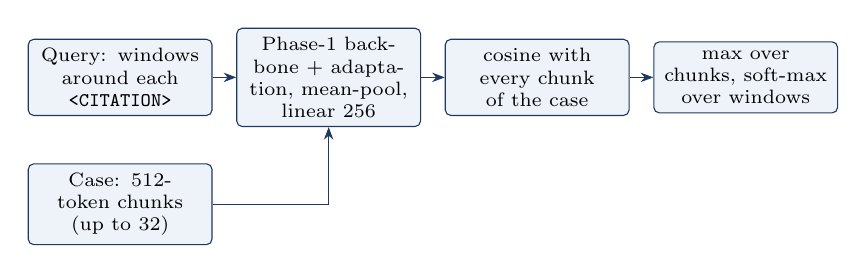
\begin{tikzpicture}[node distance=3mm, box/.style={draw=navy,rounded corners=2pt,fill=soft,align=center,
  font=\scriptsize,minimum height=9mm,text width=21mm}, arr/.style={-{Stealth[length=1.6mm]},navy}]
  \node[box] (a) {Query: windows around each \texttt{<CITATION>}};
  \node[box,right=of a] (b) {Phase-1 backbone + adaptation, mean-pool, linear 256};
  \node[box,right=of b] (c) {cosine with every chunk of the case};
  \node[box,right=of c] (d) {max over chunks, soft-max over windows};
  \node[box,below=6mm of a] (e) {Case: 512-token chunks (up to 32)};
  \draw[-{Stealth[length=1.6mm]},navy] (a)--(b); \draw[-{Stealth[length=1.6mm]},navy] (b)--(c); \draw[-{Stealth[length=1.6mm]},navy] (c)--(d);
  \draw[-{Stealth[length=1.6mm]},navy] (e) -| (b);
\end{tikzpicture}
\caption{Citation-window bi-encoder (\code{pcr/model.py}).}
\label{fig:model}\end{figure}
\begin{itemize}
  \item \textbf{Units}: a query is represented by its citation windows ($\pm60$ words, at most 256 tokens), a
  candidate by its 512-token chunks (32 evenly spread chunks at evaluation, 4 random chunks during training).
  Both pass through the same backbone, mean pooling and a 256-dimensional projection.
  \item \textbf{Score}: window--case similarity = maximum cosine over the case's chunks; query--case score =
  soft maximum over the query's windows (log-sum-exp, temperature 0.05).
  \item \textbf{Training}: 8 queries per step; for each, 2 gold cases and 3 hard negatives from the top 30
  non-gold cases of per-citation BM25; every query is scored against every case in the batch with a
  multi-positive InfoNCE loss \cite{oord2018cpc} (temperature 0.05, the query's own case removed).  10 epochs,
  AdamW, 5\% warm-up then cosine decay; the epoch with the best dev micro-F1@7 is kept.
  \item \textbf{Backbones}: A1 with bidirectional attention over the window or chunk, A3 (bidirectional prefix),
  A4 causal, A2 decoder states over the window (encoder output collapsed, Phase-2 finding).
\end{itemize}

\subsection{Adaptation techniques}
\begin{itemize}
  \item \textbf{Full fine-tuning} (E2; A1), learning rate $3\times10^{-5}$.
  \item \textbf{Partial fine-tuning} (E3; A4): the top 4 of 10 blocks, $10^{-4}$.
  \item \textbf{LoRMA} \cite{bihany2025lorma} (E1; A3): $W=(I+\tfrac{\alpha}{r}BA)W_0$, $r=32$, $\alpha=64$, $5\times10^{-4}$.
  \item \textbf{QLoRA} \cite{dettmers2023qlora} (E4; A2): frozen weights in 4-bit NF4, LoRA $r=32$, $5\times10^{-4}$.
  \item \textbf{IA$^3$} \cite{liu2022ia3} (E5; A3): learned rescaling of keys, values and the MLP, $3\times10^{-3}$.
  \item \textbf{Prefix tuning} \cite{li2021prefix} (E6; A1): 16 key/value positions per layer, $10^{-3}$.
  \item \textbf{Prompt tuning} \cite{lester2021prompt} (E7; A4): 20 input embeddings, $3\times10^{-3}$.
  \item \textbf{Knowledge distillation} \cite{hinton2015kd} (K1): A1 student with 4 of its 8 blocks (0, 2, 5, 7),
  fully fine-tuned with $0.5\,\mathrm{InfoNCE} + 0.5\,\mathrm{KL}$ between the teacher's and the student's
  score distributions over the batch's cases (temperature $2\tau$); teacher = E2.  K0 is the same student
  trained without the teacher.
\end{itemize}
Additional runs repeat E2, E1 and E3 with other seeds (E2b, E2c, E1b, E3b) and E2 with 6 hard negatives from
the top 50, 6 chunks per case and 4 epochs (E2d).

\subsection{Re-ranking and combination}
\begin{itemize}
  \item \textbf{Fused} (per run, \code{train.py}): z(neural) + $\lambda$ z(per-citation BM25) $-$ date penalty,
  $\lambda$ and the penalty picked on dev.
  \item \textbf{Learning to rank} (\code{stack.py}, \code{pcr/ltr.py}): LightGBM lambdarank \cite{ke2017lightgbm}
  over each query's top 100 candidates of the first stage.  Features: row and column z-scores and ranks of every
  lexical score, date difference and violation, candidate length, number of citation windows, and whether the
  candidate is itself a query.  Trained on train (3 seeds averaged), scored on dev; the test model is refit on
  train + dev.
  \item \textbf{Neural blend}: the ranker's z-scored output + $w\times$ the mean (row + column z-scored) score of
  several bi-encoder runs.  Using a neural score as a ranker \emph{feature} needs out-of-fold scores on train
  (2-fold runs F\_E2\_*); that variant (STK1) did not help.
  \item \textbf{Cross-encoder} (\code{cross\_train.py}, C1): A1 reads [citation window, ``Cited judgment:'', case
  chunk] for the two best window--chunk pairs of each (query, case) of the STK4 top 30 and is trained listwise
  (1 gold against 11 non-gold).
\end{itemize}

\subsection{Submissions}
\code{prediction.json} maps every test query id to 7 distinct ids from the test pool, best first, never the
query itself; every zip is checked against these rules when it is written.

% =====================================================================
\section{Results}
\subsection{Lexical retrieval}
\begin{table}[H]\centering\small
\caption{Lexical retrieval, micro-F1@7 (no learning).}\label{tab:ladder}
\begin{tabular}{lrr}\toprule Method & Dev & Train\\\midrule
\tabinput{tables/ladder.tex}
\bottomrule\end{tabular}\end{table}

\begin{figure}[H]\centering
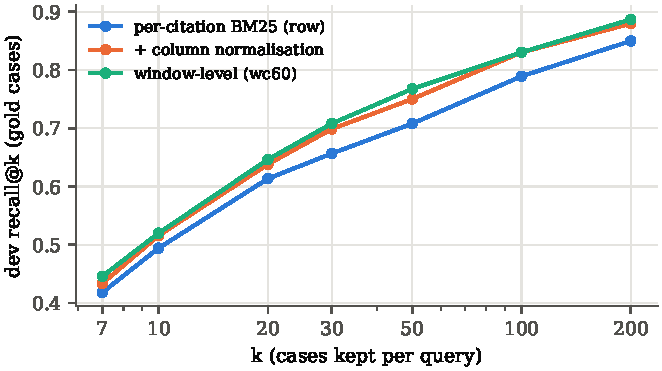
\includegraphics[width=0.7\linewidth]{figs/recall.pdf}
\caption{Share of dev gold cases among each query's top $k$ lexical candidates (window-level first stage:
\recallseven\% at $k=7$, \recallhundred\% at $k=100$).}
\label{fig:recall}\end{figure}

\subsection{Phase-1 models without training}
\begin{table}[H]\centering\small
\caption{Dev micro-F1@7 of the untrained Phase-1 backbones in the bi-encoder (mean-pooled states, no projection).}\label{tab:zs}
\begin{tabular}{lr}\toprule Backbone & Micro-F1@7\\\midrule
\tabinput{tables/zeroshot.tex}
\bottomrule\end{tabular}\end{table}

\subsection{Adaptation experiments}
\begin{table}[H]\centering
\caption{Dev results (\nqdev{} queries).  Neural = the bi-encoder alone (F1, P, R); Fused = with per-citation
BM25 and the date penalty (weights picked on dev).  Below the line: seeds and the hard-negative variant.}\label{tab:results}
\resizebox{\linewidth}{!}{\begin{tabular}{lllrrrrrrr}\toprule
Run & Arch & Method & Total & Trainable & \% & Neural F1 & P & R & Fused F1\\\midrule
\tabinput{tables/results.tex}
\bottomrule\end{tabular}}\end{table}

\begin{figure}[H]\centering
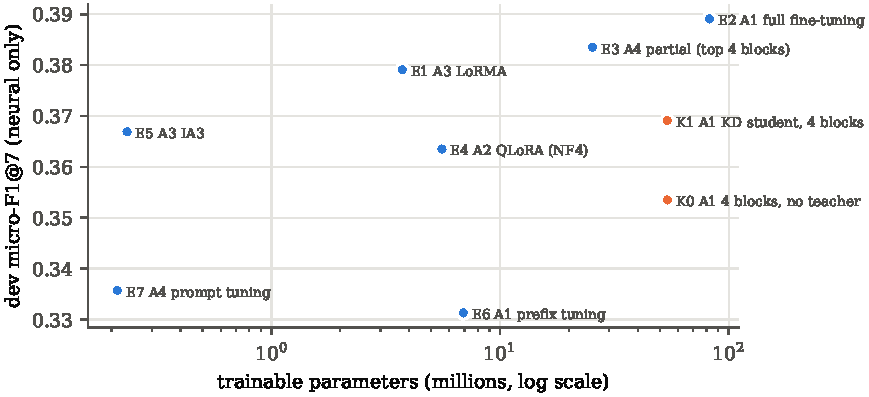
\includegraphics[width=0.85\linewidth]{figs/f1_vs_params.pdf}
\caption{Neural-only dev micro-F1@7 against trained parameters (orange: 4-block students).}
\label{fig:params}\end{figure}

\begin{figure}[H]\centering
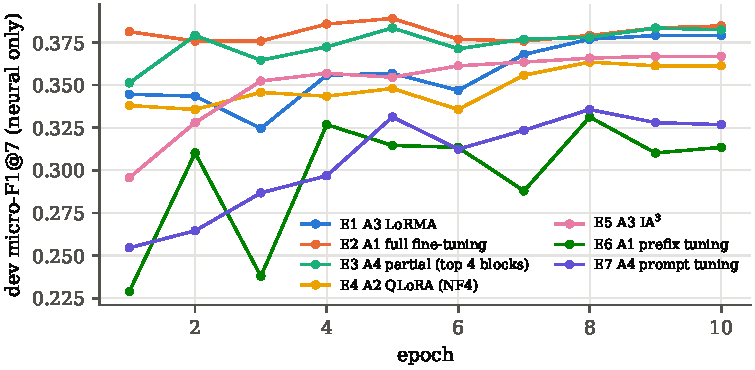
\includegraphics[width=0.85\linewidth]{figs/curves.pdf}
\caption{Neural-only dev micro-F1@7 after each epoch.}
\label{fig:curves}\end{figure}

\subsection{Knowledge distillation and efficiency}
\begin{table}[H]\centering\small
\caption{Size, compute and memory.  Encode = seconds to embed and score the whole dev split.}\label{tab:eff}
\begin{tabular}{lllrrrrr}\toprule
Run & Arch & Method & Params & Train (min) & Encode (s) & Peak GB & Ckpt MB\\\midrule
\tabinput{tables/efficiency.tex}
\bottomrule\end{tabular}\end{table}
K1 has \kdparams{} parameters against \teacherparams{} for its teacher E2 and encodes the dev split in
\kdenc{} s against \teacherenc{} s; neural-only F1 \nfKone{} (teacher \nfEtwo, same student without teacher
\nfKzero).

\subsection{Re-ranking and combination}
\begin{table}[H]\centering\small
\caption{Learning-to-rank stacks and the cross-encoder (dev).  Runs = bi-encoders blended; $w$ = blend weight.
The C1 base (STK4 alone) scores \crossbase; the cross-encoder alone re-orders the top 30 at \crossonly.}\label{tab:stacks}
\resizebox{\linewidth}{!}{\begin{tabular}{llrrrrr}\toprule
Name & Description & Runs & $w$ & F1 & P & R\\\midrule
\tabinput{tables/stacks.tex}
\bottomrule\end{tabular}}\end{table}

\subsection{Errors of the submitted system}
STK6 on dev: micro-F1@7 \finalf{} (P \finalp, R \finalr); \zerohit{} of \nqdev{} queries get no gold case.
\begin{table}[H]\centering\small
\caption{STK6 on dev by number of gold cases per query.}\label{tab:errors}
\begin{tabular}{lrrrrrr}\toprule
Gold cases & Queries & Hits in top 7 & P & R & F1 & Queries with 0 hits\\\midrule
\tabinput{tables/errors.tex}
\bottomrule\end{tabular}\end{table}

\begin{figure}[H]\centering
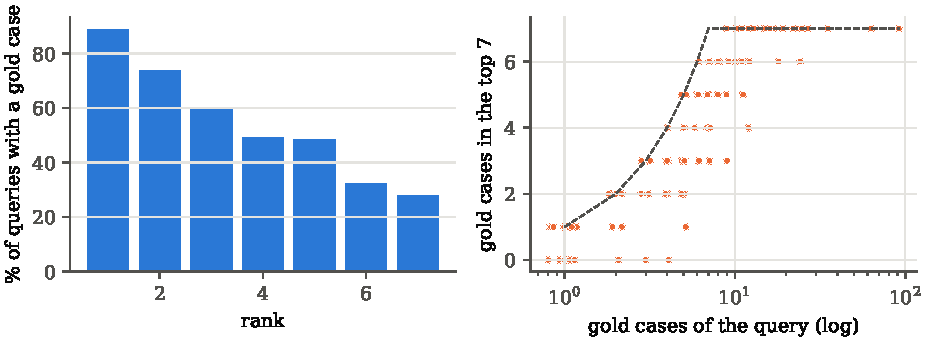
\includegraphics[width=0.95\linewidth]{figs/errors.pdf}
\caption{STK6 on dev.  Left: share of queries with a gold case at each rank.  Right: gold cases found in the
top 7 against the query's number of gold cases (dashed: the maximum for small gold sets).}
\label{fig:errors}\end{figure}

\subsection{Submission files}
\nzips{} format-checked zips are in \code{p7/submissions/}.  Uploaded first: \code{STK6\_wc\_all13}
(\stksix), \code{STK5\_all13\_w075} and \code{STK4\_rc\_blend4} (\stkfour), then one zip per technique
(\code{\_neural}: Phase-1 model only; \code{\_fused}: with BM25).
\authorbox{leaderboard scores}{Add the Codabench test micro-F1@7, precision and recall of each uploaded
submission and say which six or more count towards the requirement.}
{\scriptsize\begin{longtable}{l}\toprule File\\\midrule\endhead
\tabinput{tables/submissions.tex}
\bottomrule\end{longtable}}

% =====================================================================
\section{Analysis}
\authorbox{analysis of the results}{The course rules do not allow LLM-written result analysis.  Questions the
course asks (§13.5), with the evidence above:
\begin{itemize}
  \item How do the adaptation techniques affect retrieval quality (\autoref{tab:results}, \autoref{fig:params})?
  \item How do the Phase-1 representations transfer to PCR (\autoref{tab:zs} vs.\ \autoref{tab:results})?
  \item What is the effect of pooling and document representation (citation windows, chunk maximum,
  \autoref{tab:ladder})?
  \item What is the effect of the similarity and ranking objectives (InfoNCE, learning to rank, blending,
  \autoref{tab:stacks})?
  \item What do hard negatives and negative sampling change (E2 vs.\ E2d)?
  \item Which challenges do long legal documents pose?
  \item What are the common retrieval errors (\autoref{tab:errors}, \autoref{fig:errors})?
  \item How effective is knowledge distillation (K1 vs.\ K0 and E2, \autoref{tab:eff})?
  \item What is the trade-off between quality, size, memory and inference time?
  \item Why might a technique that works on another legal task not transfer to PCR?
\end{itemize}}

\section{Limitations and next steps}
Facts that limit the conclusions (the interpretation is the author's):
\begin{itemize}
  \item Dev has \nqdev{} queries; differences of about 0.015 micro-F1@7 are within noise.  Blend weights and
  stack variants were chosen on dev (the ranker's own settings were checked by 5-fold cross-validation on train).
  \item The submitted stacks use BM25 and the pool structure (\autoref{sec:data}); neither uses a pretrained model,
  outside data or test labels, but they are not Phase-1 models.  The \code{\_neural} zips use the Phase-1 models only.
  \item One seed for most runs; E2/E2b/E2c differ by up to 0.009.
  \item Judgment years are extracted heuristically (\autoref{sec:data}).
\end{itemize}
\authorbox{what you would do next}{With more time or compute: \ldots}

\section{Conclusions}
\authorbox{conclusions}{Summarise what you conclude from the experiments, in your own words.}

\section{Reproducibility}
\noindent{\small\begin{tabularx}{\linewidth}{l>{\raggedright\arraybackslash}X}
Lexical scores & \code{python lex.py}; \code{python lex\_wincol.py}\\
Token cache & \code{pcr/tok.py} (\code{build})\\
Experiments & \code{P=2 bash run\_queue.sh e1\_a3\_lorma e2\_a1\_full ... k1\_kd\_a1\_4l k0\_a1\_4l\_nokd}\\
One experiment & \code{python train.py --config configs/e2\_a1\_full.yaml}\\
Out-of-fold runs & \code{bash folds.sh e2\_a1\_full}\\
Final stack & \code{python stack.py --name STK6\_wc\_all13 --first wc60\_g2 --blend E2\_a1\_full ... K1\_kd\_a1\_4l --w 0.4 --refit}\\
Cross-encoder & \code{python cross\_prep.py}; \code{python cross\_train.py --config configs/c1\_a1\_cross.yaml}\\
Figures and tables & \code{python p7/report/make\_figures.py}\\
\end{tabularx}}
\authorbox{repository link}{GitHub: \url{https://github.com/...}}

\section*{LLM declaration}
\authorbox{LLM declaration (mandatory)}{Fill in the course questionnaire.  Describe honestly which parts used
an LLM assistant (for example the data pipeline, model and training code, figures and this report's
methods/results text) and which parts are your own (design decisions, hyperparameters, analysis, conclusions).}

\begin{thebibliography}{99}\small
\bibitem{bihany2025lorma} H.~Bihany, S.~Patel, A.~Modi. LoRMA: Low-rank multiplicative adaptation for LLMs. Findings of ACL 2025.
\bibitem{dettmers2023qlora} T.~Dettmers et al. QLoRA: Efficient finetuning of quantized LLMs. NeurIPS 2023.
\bibitem{hinton2015kd} G.~Hinton, O.~Vinyals, J.~Dean. Distilling the knowledge in a neural network. arXiv:1503.02531, 2015.
\bibitem{ke2017lightgbm} G.~Ke et al. LightGBM: A highly efficient gradient boosting decision tree. NeurIPS 2017.
\bibitem{lester2021prompt} B.~Lester, R.~Al-Rfou, N.~Constant. The power of scale for parameter-efficient prompt tuning. EMNLP 2021.
\bibitem{li2021prefix} X.~L.~Li, P.~Liang. Prefix-tuning: Optimizing continuous prompts for generation. ACL 2021.
\bibitem{liu2022ia3} H.~Liu et al. Few-shot parameter-efficient fine-tuning is better and cheaper than in-context learning. NeurIPS 2022.
\bibitem{oord2018cpc} A.~van den Oord, Y.~Li, O.~Vinyals. Representation learning with contrastive predictive coding. arXiv:1807.03748, 2018.
\end{thebibliography}
\end{document}
